\chapter{绪论}
\section{选题背景及意义}
随着近几年国内外自动驾驶相关技术的迅速发展,越来越多的公司开始从事自动驾驶行业的研究和商业应用探索\cite{qiuwei}。
目前从事于自动驾驶技术研发的企业主要分为三种:首先是以通用、大众等传统的车企,这类车企对于车辆的改装
拥有丰富的经验但对自动驾驶需要的相关技术比较欠缺;其次是谷歌、百度等互联网企业,这类互联网企业擅长于
自动驾驶架构研发并且工程经验相当丰富,同时积累了大量的机器学习相关的技术沉淀;另外一类是以蔚来、
小马智行等新兴的自动驾驶企业,这一类企业以视觉感知算法、规划控制算法为突破口\cite{xiaoxi}。鉴于车企
对车辆本身的研发和改装有丰富的技术沉淀而以纯自动驾驶技术为导向的新兴科技企业缺乏对车辆的技术积累,而自动
驾驶技术的落地的前提就是自动驾驶车辆的大规模量产,所以传统车企与新兴技术企业合作的模式孕育而生\cite{yty}。
到目前为止,传统车企与新兴科技企业合作项目大多集中在RoboTaxi上,并且RoboTaxi已经取得了从有到无的突破。
国外的Waymo和国内的小马智行、文远知行已经在不同的城市开启了RoboTaxi的相关业务,实现了初步商用的目标\cite{xmh}。

虽然自动驾驶的量产和商业化取得了突破性的进展,有关自动驾驶商业化应用落地的目标也初步实现,但是现有的自动驾驶
各模块的通信框架并不能满足性能上的要求以及扩展性的需求。上汽集团旗下分公司享道与Momenta(魔门塔)合作开发出
享道Robotaxi并且已经实现了上海和苏州两地的运营,但其自动驾驶内部通信架构仍然采用ROS(机器人操作系统)作为
各个功能模块的通信方法\cite{zzq}。ROS是一款主要面向与机器人研究领域的开源的元操作系统,为开发者提供了
进程间通信的相关功能并且支持分布式通信,大大简化了开发过程和开发量。
ROS存在一些无法忽视的缺点,主要缺点分为通信性能问题和扩展性问题\cite{9545285}。

一方面,自动驾驶系统中使用了种类多、数量大的传感器为自动驾驶算法模块提供车辆周围的动态信息与静态信息,
数据量达到了Gbps级别且对通信延迟非常敏感。
而ROS1提供了TCPROS和UDPROS两种通信方式实现不同进程间的通信,虽然这种通信方式在各个平台上的兼容性最好,
但此通信方式并未对同一物理机和不同物理机的进程间通信两种情况进行区分。
在同一物理机进程间通信的情况下,由于操作系统对TCP/IP协议栈的实现,发送方发送一份数据会从用户态拷贝到内核态,而接收方需要从逆向地从内核态
拷贝到用户态,通信过程中存在数据的额外拷贝的问题,在传输图像等数据量较大的数据时通信延迟会随数据量大小
呈线性增长趋势。特别地,当存在1-N通信模式(一发多收)时通信延迟会进一步上升\cite{9591166,Maruyama2016ExploringTP}。
ROS2引入了DDS(Data Distributed Service, 数据分发服务)作为其通信中间件\cite{8607261},DDS支持共享内存
方式的进程间通信,有效减少了因数据拷贝带来的通信延迟。但DDS自身对数据序列化格式单独做出了定义,与ROS2的序列化格式
并不相同,通信过程中存在多次序列化的问题\cite{Maruyama2016ExploringTP}。

另一方面,自动驾驶系统的软件架构设计正迈向SOA(Service Oriented Architecture)架构风格,
即将下载高精度地图、与云端服务器交互等功能以微服务的形式进行数据传输。
而ROS消息的发布-订阅和服务通过ROS内置的.msg和.srv文件定义并且传输过程中
都会被系统内部序列化成二进制序列的形式。ROS实现了特有的序列化方法,且此方法不能做到向前和向后兼容。
自动驾驶量产和商业化应用后自动驾驶系统需要符合SOA的架构风格,这表明自动驾驶系统需要具备与各类型终端交互的能力,而序列化方法
的兼容性成为关键,ROS的序列化方法并不适合这种场景。

因此,大多数自动驾驶公司在初期都优先采用ROS
作为自己的通信架构,但这种方法只能作为前期对产品功能开发和验证环节上的解决办法,并不适合作为最终量产
和商业化应用的技术方案。开发一款可以优化或解决上述ROS缺点的新通信方案是必经之路\cite{xml}。

综上所述,实现一个通信性能高、扩展性及兼容性强的自动驾驶通信架构不仅仅是对自动驾驶通信架构本身的优化,
还可以为将来自动驾驶系统与用户或其他终端进行通信互动打下基础。因此,本文旨在研究一个具有分布式通信能力,并且
能够根据场景自适应选择通信方式的自动驾驶运行时通信系统,优化自动驾驶通信系统通信性能,提高其多终端数据交互能力,具有一定的研究意义。

\section{国内外研究现状}
在上一节提到的自动驾驶系统中使用ROS作为通信方案的弊端在国内外从事自动驾驶的企业已经注意并且已经开始寻找替代方案。尽管ROS2的发布
修复了ROS1的一些缺点并且优化了整个通信链路的性能和稳定性,但是自研通信架构已经成为自动驾驶行业的主流。百度、博世、大陆、Autoware基金会等
都对通信架构开始了研究,在产品上用自研架构取代了ROS。虽然自研架构的路线纷纷被各家企业认可,但是这并不意味着自动驾驶行业完全抛弃了ROS,
从各大企业发布的自研通信架构可以看出其中有部分思想和实现方法依然借鉴或沿用了ROS的相关思路,大部分自研的通信框架
保留了ROS中发布-订阅的通信模式并且也都提供类似于ROS中服务(ROS Service)的相关功能。
\subsection{国内研究现状}
2019年,国内的百度公司为旗下的自动驾驶业务线Apollo研究并发布了一套自研的分布式通信框架,即CyberRT。CyberRT是
一套以ROS为参考并且致力于优化ROS缺陷,做到高并发、低延迟和高吞吐的通信系统,
提供了类似于ROS中的订阅者(Subscriber)、发布者(Publisher)和服务(Service)的通信角色。
CyberRT在设计中采用了分层次开发方法,涵盖了从最上层提供给用户的相关接口到最下层的通信方法,用户
只需要关注最上层API的应用而无需关注框架的内部实现。同时,分层次的设计方法使得整个框架
的功能耦合度很低,其架构如图\ref{cyberrt_structure}所示\cite{cyberrt}。
\begin{figure}[H]
  \centering
  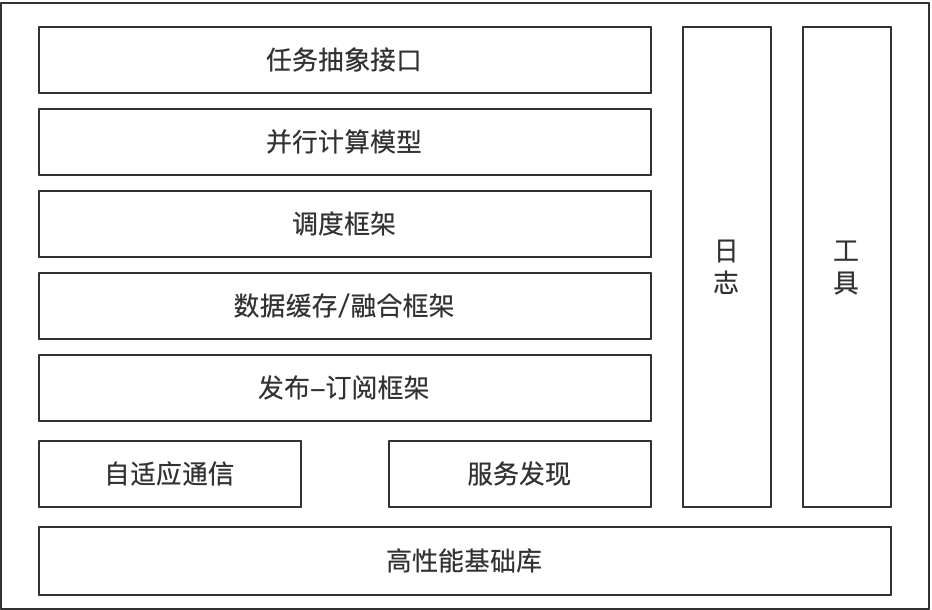
\includegraphics[width=0.65\textwidth]{cyberrt_structure.png}
  \caption{CyberRT架构图}
  \label{cyberrt_structure}
\end{figure}
根据系统的架构图可以得出CyberRT将整个通信系统分成了6层,下文将选取任务抽象层、调度层、数据通信层
和服务发现层进行论述:
\begin{enumerate}
  \item 任务抽象层:该层的主要功能为向用户提供注册订阅者、发布者以及服务的接口,用户通过该接口
  可以快速将需要接收和发布的话题在通信节点内进行注册,如果需要注册供其他通信节点调用的服务,也
  可以一起注册在节点中。当用户注册完所有的通信功能后,一个通信节点就被调度层加载到系统内与其他
  节点进行数据交互和服务调用。在注册时,API内部会自动获取该节点的实际IP地址、端口号和进程号,
  下层根据这些数据选择通信方式。
  \item 调度层:该层的功能是将任务抽象层中用户自定义的通信节点加载到调度队列中,调度策略默认是
  基于数据驱动,当某个通信节点收到了某条信息或需要发送某条信息则将唤醒该节点并执行程序。该层也支持
  基于优先级的调度策略,当通信节点需要更高优先级来进行任务调度时用户可以使用该种调度策略。
  \item 数据通信层:该层的功能是通过注册在系统中的话题,找到匹配的发布者和订阅者并根据实际情况
  选择使用共享内存或网络来进行数据通信。具体方法是:根据某一个话题匹配到发布或订阅该话题的数个
  发布者和订阅者,这些发布者或订阅者内部都携带用户注册时程序所在机器上的IP地址、进程号和端口号。
  通过比较这三个数据可以知道节点之间是否在同一台物理机上或处于不同的物理机上,如果处于同一台物理机上
  则选择共享内存的通信方式,如果不在同一台物理机上则选择网络通信。
  \item 服务发现层:CyberRT支持分布式通信,分布式通信代表着系统通信节点的拓扑网络会动态改变,
  而每个节点的服务也会动态变化,此情况下保持所有通信节点能正确接收到网络拓扑的变化并且更新自身的
  通信网络至最新状态。该层最重要的功能是满足了分布式通信的最基本需求根据动态的通信拓扑去更新
  通信网络中每一个节点的通信状态。
\end{enumerate}
\subsection{国外研究现状}
Edwin Olson等人在2010年提出了名为LCM\cite{2010LCM}的自动驾驶通信系统,该通信系统基于UDP多播方式实现了
发布-订阅的通信模式。该系统中发布者发送的数据会通过UDP多播传输至每一个订阅者,无论订阅者是否订阅了对应的话题。
订阅者需要丢弃不属于自身订阅的数据,造成了大量的资源消耗。

Neil Dantam等人在2012年弃用了基于网络的进程间通信方式,将共享内存作为进程间通信方式,并将该方式集成到
名为Ach\cite{6651538}的通信系统并运用于自动驾驶等复杂机器人应用领域。Ach系统通过使用共享内存的进程间通信方式
避免了使用TCP通信带来的队头阻塞问题(Head-of-Line Blocking Problem),有效减少了TCP有序传输机制下
数据传输过程中出现乱序而带来的阻塞延迟\cite{8863328}。

Wei Liu等人在2020年结合自动驾驶系统各节点信息流传递特点给出了ROS的通信延迟实验结果,并提出了基于共享内存的
Z-framework\cite{2020memory}。该框架使用共享内存作为进程间通信手段,有效地降低了ROS在进程间通信延迟方面
的缺陷。但该框架存在读者或写者崩溃时整个共享内存块将无法被再次使用最终无法完成通信。


罗伯特·博世公司自动驾驶部门开发了一款专注于基于共享内存实现进程间通信的自动驾驶通信中间件iceoryx(冰羚),
该中间件由Eclipse在2021年开源并面向行业内提供自动驾驶系统通信方案。
iceoryx和CyberRT非常类似,都采用了发布-订阅的通信模型和服务发现机制。该中间件的特点是对共享内存的
同步方法做出了改进。传统的共享内存数据同步的方法是利用操作系统提供的信号量或锁来保证临界资源的安全性,但这种方式的缺点是
信号量和锁的粒度太大,不利于提高程序的并发性。而iceoryx通过原子操作来实现了基于无锁队列的共享内存数据结构,
这使得中间件的并发性和吞吐量相比于传统的使用锁来实现数据同步的通信方法获得了比较大的提升\cite{iceoryx}。

虽然iceoryx的进程间通信性能非常好,但缺点是该通信中间件不支持分布式通信,这就意味着使用此中间件就无法完成跨机器
的通信。但作为进程间通信中间件本身而言,它的优点也是不容忽视的。德国大陆公司开源的eCAL自动驾驶通信
中间件就将iceoyrx作为进程间通信的子模块,而eCAL自身实现了网络通信的功能。不仅eCAL使用了iceoryx作为
进程间通信的实现,ROS2、Cyclone DDS等分布式通信系统也都使用了iceoryx\cite{ecal}。


通过上文对国内外研究现状的阐述可以发现,目前国内外自动驾驶通信系统都采用共享内存作为进程间通信的方式。但
共享内存使用起来有一定的难度,需要考虑到数据同步的问题以及如何进行异常处理。常用的组织共享内存的数据结构为
环形缓冲区(RingBuffer)。该数据结构将固定大小的共享内存区切分成n个固定大小的数据块,将其从0到n-1进行编号,同时维护写入序号和读取序号。数据块是循环使用的,向共享内存写入数据时
会使用满足条件的最小编号的数据块,并且写入完成后会将下一个可以使用的编号自增,当编号是n-1的数据块被写入数据后,会再次在编号为
0的数据块写入数据。该数据结构为了实现数据的同步,将每个数据块看作为一个临界资源,当有发布者写或
订阅者读都会尝试请求锁并获得某个数据块的访问权限进行读或写,确保不会发生脏读和脏写的情况。
如图\ref{ringbuffer}\cite{9235068}所示,
\begin{figure}[htb]
  \centering
  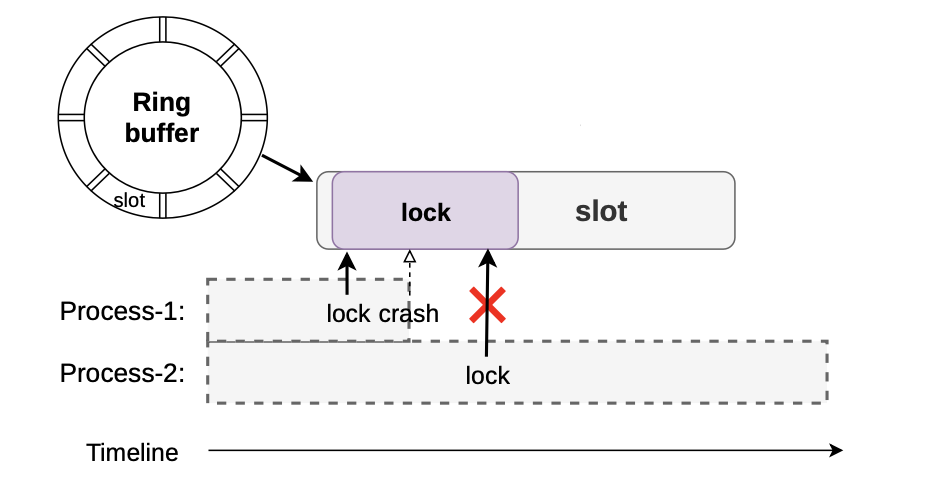
\includegraphics[width=0.65\textwidth]{1-2.png}
  \caption{环形缓冲区多进程不安全性}
  \label{ringbuffer}
\end{figure}
但此数据同步方法并不能保证程序在异常退出时能够及时地释放资源,当数据发布者在获得了某个数据块的锁并且正在写入数据时由于异常提前
终止了进程,并不会释放已经获得的锁,导致其他的发布者无法获得数据块的写入权限从而发生死锁,系统将无法完成数据通信。同样地,
当数据订阅者在读取数据时异常终止进程导致读取序号无法正常更新,发布者在写入数据时最终触发缓冲区已满的情况,出现无法写入数据的情况。

另一个不容忽视的问题是服务发现机制对系统性能影响。对于自动驾驶系统使用场景来说,通信节点存在动态增减的情况,所以需要
服务发现保证通信节点间及时发现新增节点或被删除的节点。ROS1提供了中心化的服务发现机制以同步网络内的节点和话题并且
控制节点的生命周期,称Master节点。该设计在Master节点异常终止情况下无法保证正常工作;ROS2选用了去中心化的服务发现
机制,每个通信节点保存所有的节点和话题信息。该设计下,通信节点的运行状态由心跳包判定,当节点数量达到数百个时
会消耗大量处理器资源\cite{9355690}。


\section{论文主要工作与特色}
本论文主要研究自动驾驶运行时通信系统,根据自动驾驶通信系统的研究现状,将进程间通信技术和网络
通信技术结合起来,提出基于共享内存、ZeroMQ、RPC和序列化技术的自动驾驶运行时通信系统设计方案并进行具体
实现。与现有的自动驾驶系统通信系统不同的是,本文将实现一个支持网络通信(ZeroMQ)、进程间通信
(共享内存)和进程内通信的发布-订阅通信模式和支持服务端客户端请求-应答的通信模式的自动驾驶运行时通信系统。本系统特色如下:
\begin{enumerate}
  \item 架构上遵循模块化的设计原则将各个不同功能模块解耦,使得整个系统开发与维护的难度降低,同时模块化的设计思路让系统拥有
  快速集成和易于定制化的特点,只需要修改相关编译选项即可完成功能模块的插拔。
  \item 完全自适应的通信方式,通信双方无需制定某个特定的通信方式,通信方式的选择完全由通信系统本身决定选择进程内通信、进程间通信或
  网络通信,极大地降低了通信延迟。
  \item 系统提供了消息生成器工具,该工具向用户提供了与ROS一样的开发流程,用户可以快速自定义消息格式并通过脚本自动化生成代码,
  无需额外开发序列化与反序列化代码。  
\end{enumerate}

整个项目设计与实现的过程中,本人主要工作如下:
\begin{enumerate}
  \item 调研基于共享内存的进程间通信方式,对共享内存中的地址空间进行分配与使用,独立设计了基于网络同步的高鲁棒性共享内存读写模型,
  同时满足了自动驾驶通信高实时性的要求。
  \item 对系统现有的中心节点方案作出改进,独立设计了一种通过进程监控和实时备份数据的中心节点方案,提高了中心节点的鲁棒性,
  保证了整个通信系统网络拓扑的可靠性;设计查询通信系统网络拓扑功能,为数采模块提供了准确了需要录制的数据,提高了数据回流的效率,各算法
  模块也能够根据网络拓扑调整相应的算法。
  \item 参与系统中通信单元模块、服务模块、服务发现模块和通信传输模块的开发工作,在四个模块中融合了DDS中通信域的概念并负责
  优化内存的申请以及减少额外的内存拷贝操作。
  \item 独立设计了一种测试通信系统实时性的方法,通过多种场景准确反映通信系统的通信延迟数据。
\end{enumerate}

\section{章节安排}
本论文的章节结构如图\ref{thesis_structure}所示,章节安排如下:

第一章,绪论。本章首先对自动驾驶中通信系统现有的应用场景和缺陷进行了相关介绍,具体包括本论文的
研究背景介绍以及对研究现状的介绍与分析,其次说明了本论文的研究意义以及本文的主要工作内容。

第二章,相关技术介绍。本章主要介绍了网络通信中间件ZeroMQ、序列化技术Protocol Buffer、远程服务调用
技术RPC以及共享内存,阐述并论证为何选用上述技术,以及如何将上述技术应用到本论文的研究对象中。

第三章,自动驾驶运行时通信系统需求分析。本章针对自动驾驶系统运行时通信系统的特点,导出本文自动驾驶运行时通信系统的功能性需求和非功能性需求。

第四章,自动驾驶运行时通信系统概要设计。本章结合架构图和活动图对自动驾驶系统中自动驾驶运行时通信系统进行整体的设计,
结合流程图、时序图对通信系统中各个模块的设计进行阐述。

第五章,自动驾驶运行时通信系统详细设计与实现。本章结合类图与时序图详细叙述本文如何实现自动驾驶运行时通信系统,并着重阐述前文提出的
共享内存数据结构以及服务发现机制的不足之处的改进方法。

第六章,测试与分析。本章通过功能测试来检查系统是否达到本文提出的功能性需求;通过数据大小、数据发布频率、通信参与者数量等多个维度
对展开对本文设计的通信系统进行性能测试,将通信延迟等性能指标与同类产品进行比较,并对测试结果进行详细分析。

第七章,总结与展望。总结本文完成的研究内容并分析系统中存在的不足之处以及对本系统的展望。

\begin{figure}[H]
  \centering
  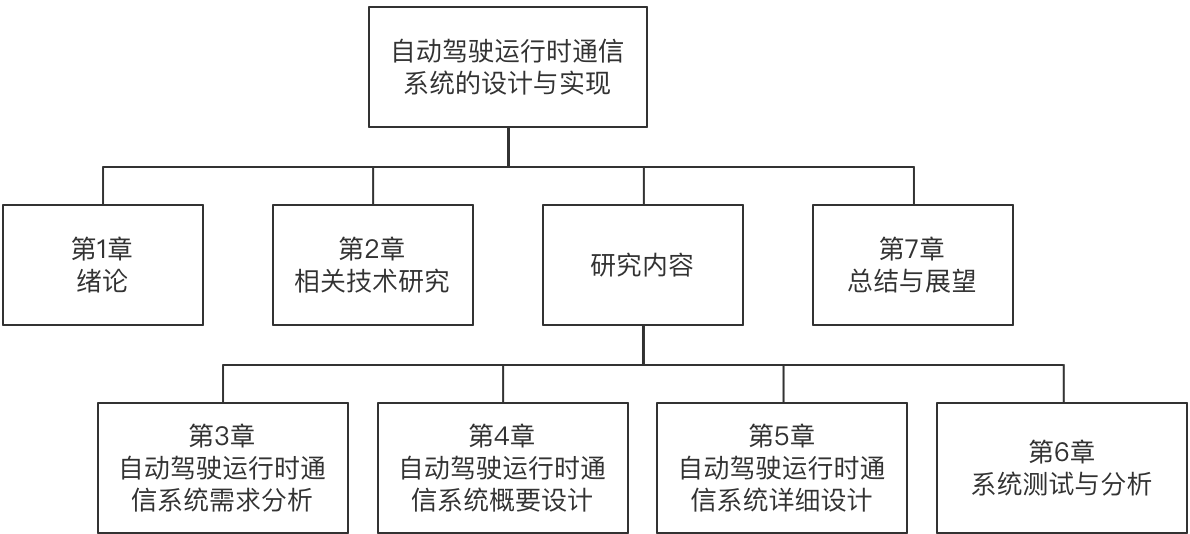
\includegraphics[width=0.78\textwidth]{thesis_structure.png}
  \caption{论文章节结构图}
  \label{thesis_structure}
\end{figure}






